\documentclass[aspectratio=169]{beamer}

\usepackage{Archivo}
\renewcommand{\sfdefault}{\rmdefault}
\usepackage{graphicx}
\usepackage{tikz}
\usetikzlibrary{calc,positioning}
\tikzset{
  invisible/.style={opacity=0, text opacity=0},
  visible on/.style={alt={#1{}{invisible}}},
  alt/.code args={<#1>#2#3}{%
    \alt<#1>{\pgfkeysalso{#2}}{\pgfkeysalso{#3}}%
  },
}
\usepackage[most]{tcolorbox}
\usepackage{listings}

%% ---- Superteam Poland brand colors ----
\definecolor{stpldark}{HTML}{0B0E0F}   % near-black background
\definecolor{stplcard}{HTML}{161A1B}   % card / block surface
\definecolor{stplborder}{HTML}{1E2526}  % subtle track color for progress bar
\definecolor{stplred}{HTML}{DC143C}    % brand crimson red
\definecolor{stplwhite}{HTML}{FFFFFF}  % white
\definecolor{stplmuted}{HTML}{8A9BA8}  % muted / secondary text

\usetheme{default}
\setbeamersize{text margin left=0.85cm, text margin right=0.85cm}

%% ---- Background & base text ----
\setbeamercolor{background canvas}{bg=stpldark}
\setbeamercolor{normal text}{fg=stplwhite, bg=stpldark}
\usebeamercolor{normal text}

%% ---- Background image helpers ----
\newcommand{\stpldefaultbg}{%
  \setbeamertemplate{background}{%
    \begin{tikzpicture}[remember picture, overlay]
      \node[at=(current page.center), inner sep=0pt] {%
        \includegraphics[width=\paperwidth,height=\paperheight]{images/bg-default.png}%
      };
      \fill[stplborder]
        (current page.north west) rectangle
        ([yshift=-2.5pt]current page.north east);
      \pgfmathsetmacro{\stplprog}{\insertframenumber/\inserttotalframenumber}
      \fill[stplred]
        (current page.north west) rectangle
        ($(current page.north west)+(\stplprog\paperwidth,-2.5pt)$);
    \end{tikzpicture}%
  }%
}
\newcommand{\stplherobg}{%
  \setbeamertemplate{background}{%
    \includegraphics[width=\paperwidth,height=\paperheight]{images/bg-hero.png}%
  }%
}
\stpldefaultbg

%% ---- Structure ----
\setbeamercolor{structure}{fg=stplred}

%% ---- Title slide metadata ----
\setbeamercolor{title}{fg=stplwhite}
\setbeamercolor{subtitle}{fg=stplred}
\setbeamercolor{author}{fg=stplwhite}
\setbeamercolor{institute}{fg=stplmuted}
\setbeamercolor{date}{fg=stplmuted}

%% ---- Frame title: flat, no box background ----
\setbeamercolor{frametitle}{fg=stplwhite, bg=}
\setbeamerfont{frametitle}{size=\large, series=\bfseries}
\setbeamertemplate{frametitle}{%
  \vspace{0.35cm}%
  {\centering\insertframetitle\par}%
  \nointerlineskip\vspace{0.18cm}%
  \hfil{\color{stplred}\rule{2.2cm}{1.5pt}}\hfil\par%
}



%% ---- Incremental reveals ----
%% Bullets reveal one at a time by default. See style.md §4.5 for the two
%% per-frame opt-outs (static frame: `\begin{frame}<1>{...}`; manually
%% choreographed frame: `\beamerdefaultoverlayspecification{}` at frame top).
\beamerdefaultoverlayspecification{<+->}

%% ---- Bullet items ----
\setbeamercolor{itemize item}{fg=stplred}
\setbeamercolor{itemize subitem}{fg=stplmuted}
\setbeamercolor{itemize subsubitem}{fg=stplmuted}
\setbeamertemplate{itemize item}{\bfseries\textendash}
\setbeamertemplate{itemize subitem}{\small\textendash}
\setbeamercolor{enumerate item}{fg=stplred}
\setbeamercolor{enumerate subitem}{fg=stplmuted}
\setbeamertemplate{enumerate item}{\textcolor{stplred}{\bfseries\insertenumlabel.}}
\setbeamertemplate{enumerate subitem}{\textcolor{stplmuted}{\small\insertenumlabel.}}

%% ---- Blocks (flat left-accent via tcolorbox) ----
\tcbset{
  stplbase/.style={
    enhanced, breakable,
    colback=stplcard, coltext=stplwhite,
    coltitle=stplwhite, fonttitle=\bfseries,
    boxrule=0pt, leftrule=3pt,
    arc=0pt, outer arc=0pt,
    top=5pt, bottom=5pt, left=7pt, right=7pt,
    toptitle=4pt, bottomtitle=4pt,
    titlerule=0pt,
  },
}
\renewenvironment{block}[1]{%
  \pause%
  \begin{tcolorbox}[stplbase, colframe=stplred, title={#1}]%
}{%
  \end{tcolorbox}%
}
\renewenvironment{alertblock}[1]{%
  \pause%
  \begin{tcolorbox}[stplbase, colframe=stplred!75!black,
    colback=stplred!10!stplcard, title={#1}]%
}{%
  \end{tcolorbox}%
}
\renewenvironment{exampleblock}[1]{%
  \pause%
  \begin{tcolorbox}[stplbase, colframe=stplmuted, title={#1}]%
}{%
  \end{tcolorbox}%
}

%% ---- Code listings (Rust + Anchor) ----
\lstdefinelanguage{Rust}{
  keywords={fn,pub,struct,impl,trait,let,mut,self,Self,match,return,for,in,
            if,else,enum,use,mod,as,where,Option,Result,Some,None,Ok,Err,
            u8,u16,u32,u64,i64,u128,bool,String,Vec,Pubkey,Context,msg,vec,
            Account,Signer,Program,System,has_one,init,payer,space,seeds,bump},
  morecomment=[l]{//},
  morestring=[b]",
  sensitive=true,
}
\lstset{
  basicstyle=\ttfamily\scriptsize\color{stplwhite},
  backgroundcolor=\color{stplcard},
  keywordstyle=\color{stplred}\bfseries,
  commentstyle=\color{stplmuted},
  stringstyle=\color{stplmuted},
  showstringspaces=false,
  keepspaces=true,
  columns=fixed,
  basewidth=0.46em,
  frame=leftline,
  framerule=2pt,
  rulecolor=\color{stplred},
  xleftmargin=0.6em,
  aboveskip=0.4em,
  belowskip=0.2em,
  language=Rust,
  escapeinside={(*@}{@*)},
}

%% ---- Code reveal card (line-synced to bullets) ----
%% A block-styled card WITHOUT the block's auto-\pause, so it is visible from
%% the current overlay and its code lines can reveal in step with the itemize
%% bullets via (*@\onslide<k->@*) markers. The listing drops its own
%% background/frame (style=reveal) so the solid card shows through instead of
%% the per-line background going ragged as lines are covered.
\newtcolorbox{codeblock}[1]{stplbase, colframe=stplred, title={#1}}
\lstdefinestyle{reveal}{backgroundcolor={}, frame=none, xleftmargin=0pt,
  aboveskip=0pt, belowskip=0pt}

%% ---- Table of contents ----
\setbeamercolor{section in toc}{fg=stplwhite}
\setbeamercolor{subsection in toc}{fg=stplmuted}
\setbeamertemplate{section in toc}{%
  {\color{stplred}\textbf{\textendash}}\hspace{0.5em}\inserttocsection%
}

%% ---- Footline: minimal ----
%% Transparent bg so the background image shows through (normal text has
%% bg=stpldark, which would paint a flat band over the image's bottom glow).
\setbeamercolor{footline}{fg=stplwhite, bg=}
\setbeamertemplate{footline}{%
  \begin{beamercolorbox}[wd=\paperwidth, ht=0pt, dp=0.55cm]{footline}%
    \hspace{0.85cm}%
    \raisebox{-0.42cm}{\includegraphics[height=0.42cm]{images/stpl-logo.png}}%
    \hfill%
    \raisebox{-0.24cm}{\textcolor{stplmuted}{\tiny\insertframenumber\,/\,\inserttotalframenumber}}%
    \hspace{0.85cm}%
  \end{beamercolorbox}%
}
\setbeamertemplate{navigation symbols}{}

%% ---- Title page defaults (decks may override) ----
\date{\the\year}

%% ---- Title frame helper (uses hero background) ----
\newcommand{\maketitleframe}{%
  \stplherobg
  \begin{frame}[plain]%
    \titlepage%
  \end{frame}%
  \stpldefaultbg
}

%% ---- Section divider slides ----
\AtBeginSection[]{%
  \stplherobg
  \begin{frame}[plain]
    \begin{tikzpicture}[remember picture, overlay]
      \fill[stplred, opacity=0.07]
        ([xshift=-2.5cm]current page.east) circle (5.5cm);
      \fill[stplred]
        (current page.north west) rectangle ([xshift=5pt]current page.south west);
    \end{tikzpicture}%
    \vfill
    \hspace{0.1\paperwidth}%
    \begin{minipage}{0.8\paperwidth}
      \textcolor{stplmuted}{\small Section \thesection}\\[0.35cm]
      {\color{stplwhite}\LARGE\bfseries\insertsectionhead}\\[0.25cm]
      {\color{stplred}\rule{3cm}{1.5pt}}
    \end{minipage}%
    \vfill
  \end{frame}%
  \stpldefaultbg
}

%% ---- Title page ----
\setbeamertemplate{title page}{%
  \begin{tikzpicture}[remember picture, overlay]
    \fill[stplred]
      (current page.north west) rectangle ([xshift=5pt]current page.south west);
    \fill[stplred, opacity=0.07]
      ([xshift=-3cm,yshift=3cm]current page.north east) circle (5.5cm);
    \fill[stplred, opacity=0.04]
      ([yshift=-1.5cm]current page.south east) circle (3.5cm);
  \end{tikzpicture}%
  \vfill
  \hspace{0.08\paperwidth}%
  \begin{minipage}{0.85\paperwidth}
    \includegraphics[width=3cm]{images/stpl-logo.png}\par
    \vspace{0.8cm}
    {\usebeamerfont{title}\usebeamercolor[fg]{title}\inserttitle}\par
    \vspace{0.2cm}
    {\color{stplred}\rule{3cm}{1.5pt}}\par
    \vspace{0.3cm}
    {\usebeamerfont{subtitle}\usebeamercolor[fg]{subtitle}\insertsubtitle}\par
    \vspace{0.65cm}
    {\usebeamerfont{author}\usebeamercolor[fg]{author}\insertauthor}\par
    \vspace{0.12cm}
    {\small\textcolor{stplmuted}{\insertinstitute\enspace·\enspace\insertdate}}
  \end{minipage}%
  \vfill
}


\usepackage[utf8]{inputenc}
\usepackage[T1]{fontenc}
\usepackage{qrcode}

%% QR na ciemnym tle: czarne moduly na bialym kartoniku -- odwrocony kontrast
%% bywa nieczytelny dla czesci skanerow.
\newcommand{\stplqr}[3]{%
  \begin{minipage}[t]{0.44\textwidth}
    \centering
    \colorbox{white}{\color{black}\qrcode[height=2cm, padding]{#1}}\\[0.2cm]
    {\small\textbf{#2}}\\[0.05cm]
    \textcolor{stplmuted}{\tiny #3}
  \end{minipage}%
}

%% Deck-local listing keywords: control flow and scalar types that the shared
%% Anchor-oriented keyword set in preamble.tex does not cover.
\lstset{morekeywords={loop,while,break,continue,const,static,true,false,
                      char,f32,f64,i8,i16,i32,i128,isize,usize,u128,len,rev}}

\title{Wspólne koncepcje}
\subtitle{The Rust Book, rozdział 3 --- zmienne, typy, funkcje, sterowanie}
\author{Mateusz Zając}
\institute{Kurs Rusta}

\begin{document}

\maketitleframe

\begin{frame}{O mnie}
  \begin{itemize}
    \item \textbf{Rust} od pięciu lat --- blockchain, kryptografia, systemy rozproszone
    \item Produkcyjne DeFi, systemy dowodów zero-knowledge, rdzeń łańcucha bloków
    \item Poprawność stanu i \textbf{odporność na awarie} na działającej sieci
    \item Obecnie DevRel w \textbf{Superteam Poland}
  \end{itemize}
  \vspace{0.35cm}
  \begin{center}
    \textcolor{stplmuted}{\small github.com/matzayonc}
  \end{center}
\end{frame}

\begin{frame}{Plan}
  \tableofcontents
\end{frame}

% ================================================================
\section{Zmienne}

\begin{frame}[fragile]{Niemutowalność}
  \begin{itemize}
    \item Zmienna jest domyślnie \textbf{niemutowalna} --- raz przypisana, zostaje
    \item Ponowne przypisanie to błąd kompilacji, nie awaria w czasie działania
    \item Jak \texttt{const} z JavaScriptu, ale obejmuje również wnętrze wartości
    \item \texttt{mut} to jawna zgoda na zmianę --- widoczna dla czytelnika kodu
  \end{itemize}
  \begin{block}{let a let mut}
\begin{lstlisting}
let x = 5;
x = 6;          // error: cannot assign twice to immutable variable

let mut y = 5;
y = 6;          // OK
\end{lstlisting}
  \end{block}
\end{frame}

\begin{frame}[fragile]{Stałe}
  \begin{itemize}
    \item \texttt{const} jest niemutowalna zawsze --- \texttt{mut} jest tu zabronione
    \item Typ trzeba podać jawnie, a wartość musi być znana w czasie kompilacji
    \item Stała może żyć w zasięgu globalnym, poza jakąkolwiek funkcją
    \item Konwencja nazw to \textbf{wielkie litery} rozdzielone podkreśleniem
  \end{itemize}
  \begin{block}{Wyrażenie liczone przez kompilator}
\begin{lstlisting}
const TRZY_GODZINY_W_SEKUNDACH: u32 = 60 * 60 * 3;

// w binarce jest juz 10800 -- mnozenia nie ma w czasie dzialania
\end{lstlisting}
  \end{block}
\end{frame}

\begin{frame}[fragile]{Przesłanianie}
  \begin{itemize}
    \item Powtórzone \texttt{let} tworzy \textbf{nową} zmienną, a nie zmienia starej
    \item \textbf{Przesłanianie} (shadowing) pozwala zmienić typ; \texttt{mut} na to nie pozwala
    \item Przesłonięcie kończy się razem z zasięgiem, w którym powstało
    \item Typowe użycie: konwersja danych wejściowych bez drugiej nazwy
  \end{itemize}
  \begin{block}{Dwie różne decyzje}
\begin{lstlisting}
let spacje = "   ";
let spacje = spacje.len();   // &str -> usize, nowa zmienna

let mut spacje = "   ";
spacje = spacje.len();       // error: mismatched types
\end{lstlisting}
  \end{block}
\end{frame}

% ================================================================
\section{Typy danych}

\begin{frame}[fragile]{Typy skalarne}
  \begin{itemize}
    \item Rust jest statycznie typowany --- typ musi być znany w czasie kompilacji
    \item Cztery rodziny skalarne: całkowite, zmiennoprzecinkowe, \texttt{bool}, \texttt{char}
    \item Bez adnotacji kompilator przyjmuje \textbf{\texttt{i32}} i \textbf{\texttt{f64}}
    \item \texttt{char} zajmuje cztery bajty --- mieści każdy znak Unicode, nie tylko ASCII
  \end{itemize}
  \begin{block}{Cztery rodziny}
\begin{lstlisting}
let calkowita: i32  = -42;    // i8 i16 i32 i64 i128 isize (+ u8 .. usize)
let ulamek:    f64  = 2.5;    // f32 f64
let flaga:     bool = true;
let znak:      char = 'A';    // 4 bajty, wartosc skalarna Unicode
\end{lstlisting}
  \end{block}
\end{frame}

\begin{frame}[fragile]{Przepełnienie}
  \begin{itemize}
    \item \texttt{u8} mieści zakres 0--255 --- wartość 256 nie ma się gdzie zmieścić
    \item Kompilacja \texttt{debug}: program \textbf{panikuje} i zatrzymuje się z komunikatem
    \item Kompilacja \texttt{release}: wartość cicho się zawija i 256 staje się 0
    \item Ten sam kod zachowuje się inaczej w obu trybach --- decyzja musi być jawna
  \end{itemize}
  \begin{alertblock}{Jawna arytmetyka}
\begin{lstlisting}
let a: u8 = 255;
let b = a + 1;                // debug: panic, release: 0

let c = a.checked_add(1);     // None zamiast paniki
let d = a.saturating_add(1);  // 255 -- zatrzymanie na granicy
\end{lstlisting}
  \end{alertblock}
\end{frame}

\begin{frame}[fragile]{Krotki}
  \begin{itemize}
    \item \textbf{Krotka} (tuple) łączy wartości \textbf{różnych} typów w jedną całość
    \item Długość jest stała --- po utworzeniu krotka nie rośnie ani nie maleje
    \item Rozpakowanie odbywa się wzorcem, dostęp do pola --- indeksem po kropce
    \item Pusta krotka \texttt{()} to typ jednostkowy: wartość funkcji, która nic nie zwraca
  \end{itemize}
  \begin{block}{Rozpakowanie i indeks}
\begin{lstlisting}
let krotka: (i32, f64, char) = (500, 6.4, 'A');

let (x, y, z) = krotka;     // rozpakowanie wzorcem
let pierwszy  = krotka.0;   // dostep po indeksie
\end{lstlisting}
  \end{block}
\end{frame}

\begin{frame}[fragile]{Tablice}
  \begin{itemize}
    \item \textbf{Tablica} (array) to stała liczba elementów \textbf{jednego} typu
    \item Długość jest częścią typu --- \texttt{[i32; 5]} to inny typ niż \texttt{[i32; 6]}
    \item Cała tablica leży na stosie, bo jej rozmiar jest znany w czasie kompilacji
    \item Indeks poza zakresem to panika, a nie odczyt przypadkowej pamięci
  \end{itemize}
  \vspace{-0.05cm}
  \begin{center}
    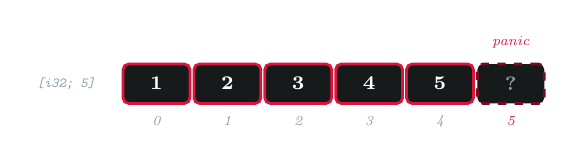
\begin{tikzpicture}[
        every node/.style={font=\scriptsize\bfseries},
        cell/.style={
          draw=stplred, line width=1pt,
          fill=stplcard, text=stplwhite,
          rounded corners=2pt,
          minimum width=0.85cm, minimum height=0.5cm, align=center,
        },
        idx/.style={font=\tiny\itshape, text=stplmuted},
      ]
      \foreach \v/\i in {1/0, 2/1, 3/2, 4/3, 5/4} {
        \node[cell] (c\i) at (\i*0.9, 0) {\v};
        \node[idx]  at (\i*0.9, -0.48) {\i};
      }
      \node[cell, draw=stplred!55!black, dashed, text=stplmuted] (out) at (4.5, 0) {?};
      \node[idx, text=stplred] at (4.5, -0.48) {5};
      \node[font=\tiny\itshape, text=stplred] at (4.5, 0.52) {panic};
      \node[idx] at (-1.15, 0) {\texttt{[i32; 5]}};
    \end{tikzpicture}
  \end{center}
  \vspace{-0.1cm}
  \begin{block}{Zapis}
\begin{lstlisting}
let a: [i32; 5] = [1, 2, 3, 4, 5];
let zera = [0; 3];    // [0, 0, 0] -- wartosc i powtorzenie
\end{lstlisting}
  \end{block}
\end{frame}

% ================================================================
\section{Funkcje i wyrażenia}

\begin{frame}[fragile]{Funkcje}
  \begin{itemize}
    \item Definicja zaczyna się od \texttt{fn}, nazwa idzie w \texttt{snake\_case}
    \item Typ każdego parametru jest \textbf{obowiązkowy} --- kompilator nie zgaduje
    \item Kolejność definicji nie ma znaczenia; liczy się zasięg, nie miejsce w pliku
    \item \texttt{main} to punkt wejścia każdego programu wykonywalnego
  \end{itemize}
  \begin{block}{Definicja i wywołanie}
\begin{lstlisting}
fn main() {
    wypisz_sume(5, 6);          // zdefiniowana nizej -- to nie problem
}

fn wypisz_sume(x: i32, y: i32) {
    println!("{}", x + y);
}
\end{lstlisting}
  \end{block}
\end{frame}

\begin{frame}[fragile]{Wyrażenia}
  \begin{itemize}
    \item \textbf{Instrukcja} wykonuje działanie i nie zwraca żadnej wartości
    \item \textbf{Wyrażenie} oblicza się do wartości --- i takich jest w Ruście większość
    \item Blok \texttt{\{\ \}} też jest wyrażeniem: jego wartością jest ostatnie wyrażenie
    \item Średnik zamienia wyrażenie w instrukcję i \textbf{odrzuca} jego wartość
  \end{itemize}
  \begin{block}{Średnik ma znaczenie}
\begin{lstlisting}
let y = { let x = 3; x + 1  };   // y == 4
let z = { let x = 3; x + 1; };   // z == () -- wartosc odrzucona

let a = (let b = 5);             // error: let nie jest wyrazeniem
\end{lstlisting}
  \end{block}
\end{frame}

\begin{frame}[fragile]{Zwracanie wartości}
  \begin{itemize}
    \item Typ wyniku deklaruje strzałka \texttt{->}; wynik nie potrzebuje nazwy
    \item Funkcja zwraca \textbf{ostatnie wyrażenie} --- \texttt{return} służy do wyjścia wcześniej
    \item Średnik po tym wyrażeniu zmienia wynik na \texttt{()} i psuje kompilację
    \item Komunikat \texttt{mismatched types} wskazuje zwykle właśnie zgubiony średnik
  \end{itemize}
  \begin{alertblock}{Jeden znak różnicy}
\begin{lstlisting}
fn piatka() -> i32 {
    5      // brak srednika: to jest zwracana wartosc
}

fn zle() -> i32 {
    5;     // error: mismatched types -- blok zwraca ()
}
\end{lstlisting}
  \end{alertblock}
\end{frame}

\begin{frame}[fragile]{Komentarze}
  \begin{itemize}
    \item \texttt{//} komentuje do końca wiersza; dłuższy komentarz to kilka takich wierszy
    \item Komentarz nad kodem czyta się lepiej niż doklejony na końcu wiersza
    \item \texttt{///} to komentarz dokumentacyjny --- trafia do wyniku \texttt{cargo doc}
    \item Komentarz opisuje \textbf{dlaczego}, a nie \textbf{co} --- „co'' widać w kodzie
  \end{itemize}
  \begin{exampleblock}{Komentarz, który coś wnosi}
\begin{lstlisting}
// Limit sesji ustalony z zespolem bezpieczenstwa -- nie skracac.
const TRZY_GODZINY_W_SEKUNDACH: u32 = 60 * 60 * 3;
\end{lstlisting}
  \end{exampleblock}
\end{frame}

% ================================================================
\section{Sterowanie}

\begin{frame}[fragile]{Warunki}
  \begin{itemize}
    \item Warunek musi być typu \texttt{bool} --- liczba ani napis nie są „prawdziwe''
    \item Nawiasy wokół warunku są zbędne, klamry wokół gałęzi obowiązkowe
    \item \texttt{if} jest wyrażeniem, więc może stać po prawej stronie \texttt{let}
    \item Wszystkie gałęzie takiego \texttt{if} muszą zwracać \textbf{ten sam typ}
  \end{itemize}
  \begin{block}{if jako wyrażenie}
\begin{lstlisting}
let liczba = 3;
// if liczba { }   // error: expected `bool`, found integer

let opis = if liczba % 2 == 0 { "parzysta" } else { "nieparzysta" };
\end{lstlisting}
  \end{block}
\end{frame}

\begin{frame}[fragile]{Pętle}
  \begin{itemize}
    \item Trzy rodzaje: \texttt{loop} bez warunku, \texttt{while} z warunkiem, \texttt{for} po kolekcji
    \item \texttt{break} przerywa pętlę, \texttt{continue} przechodzi do następnego obiegu
    \item \texttt{loop} jest wyrażeniem --- \texttt{break} z wartością zwraca wynik z pętli
    \item Typowe zastosowanie: ponawianie operacji, która może się nie udać
  \end{itemize}
  \vspace{-0.2cm}
  \begin{center}
    \begin{tikzpicture}[
        every node/.style={font=\scriptsize\bfseries},
        b/.style={
          draw=stplred, line width=1pt,
          fill=stplcard, text=stplwhite,
          rounded corners=2pt,
          minimum width=2.2cm, minimum height=0.6cm, align=center,
        },
        o/.style={
          draw=stplmuted, line width=1pt,
          fill=stplcard, text=stplwhite,
          rounded corners=2pt,
          minimum width=1.5cm, minimum height=0.6cm, align=center,
        },
        arr/.style={-latex, draw=stplred, line width=1pt},
        lbl/.style={font=\tiny\itshape, text=stplmuted},
      ]
      \node[b] (body) at (0,0)   {ciało pętli};
      \node[o] (res)  at (4.2,0) {\texttt{wynik}};
      \draw[arr] (body) -- (res) node[midway, above, lbl] {\texttt{break} wartość};
      \draw[arr, draw=stplmuted]
        (body.north east) to[out=60, in=120, looseness=1.0] (body.north west);
      \node[lbl] at (0, 0.6) {kolejny obieg};
    \end{tikzpicture}
  \end{center}
  \vspace{-0.2cm}
  \begin{block}{loop zwraca wartość}
\begin{lstlisting}
let wynik = loop {
    licznik += 1;
    if licznik == 10 { break licznik * 2; }
};                                          // wynik == 20
\end{lstlisting}
  \end{block}
\end{frame}

\begin{frame}[fragile]{Etykiety}
  \begin{itemize}
    \item W zagnieżdżonych pętlach \texttt{break} przerywa tylko tę, w której stoi
    \item \textbf{Etykieta} zaczyna się apostrofem i stoi przed słowem \texttt{loop}
    \item \texttt{break 'nazwa} przerywa pętlę wskazaną, a nie najbliższą
    \item \texttt{continue 'nazwa} działa analogicznie dla następnego obiegu
  \end{itemize}
  \begin{block}{Wyjście z dwóch pętli naraz}
\begin{lstlisting}
'zewnetrzna: loop {
    loop {
        if licznik == 2 { break; }               // przerywa wewnetrzna
        if pozostalo == 9 { break 'zewnetrzna; } // przerywa obie
    }
}
\end{lstlisting}
  \end{block}
\end{frame}

\begin{frame}[fragile]{Pętla for}
  \begin{itemize}
    \item \texttt{while} z licznikiem wymaga ręcznego indeksu --- łatwo pomylić zakres
    \item Pomyłka w warunku kończy się paniką w czasie działania, nie błędem kompilacji
    \item \texttt{for} przechodzi po elementach kolekcji i usuwa indeks z kodu
    \item Zakres \texttt{1..4} oraz \texttt{.rev()} zastępują licznik w pętli odliczającej
  \end{itemize}
  \begin{block}{Ręcznie i idiomatycznie}
\begin{lstlisting}
let a = [10, 20, 30];

let mut i = 0;
while i < 3 { println!("{}", a[i]); i += 1; }   // recznie, ryzykownie

for element in a { println!("{}", element); }   // idiomatycznie
for i in (1..4).rev() { println!("{}", i); }    // 3, 2, 1
\end{lstlisting}
  \end{block}
\end{frame}

% ================================================================
\begin{frame}{Podsumowanie}
  \begin{enumerate}
    \item \textbf{Niemutowalność} jest domyślna --- \texttt{mut} i przesłanianie to różne decyzje
    \item Typy skalarne i złożone mają rozmiar znany w czasie \textbf{kompilacji}
    \item Prawie wszystko jest \textbf{wyrażeniem} --- średnik odrzuca wartość
    \item Funkcja zwraca ostatnie wyrażenie: bez \texttt{return} i bez średnika
    \item \texttt{if} oraz \texttt{loop} również zwracają wartości; \texttt{for} to domyślna pętla
  \end{enumerate}
  \vspace{0.2cm}
  \begin{exampleblock}{Efekt}
    Po tym rozdziale czyta się każdy program, który nie dotyka własności ---
    a własność to rozdział 4.
  \end{exampleblock}
\end{frame}

% ================================================================
\begin{frame}{Materiały}
  \begin{itemize}
    \item \textbf{The Rust Book} --- rozdział 3 w całości, razem z ćwiczeniami na końcu
    \item \textbf{Jon Gjengset} --- „Crust of Rust'': te same tematy o poziom głębiej
  \end{itemize}
  \vspace{0.35cm}
  \begin{center}
    \stplqr{https://doc.rust-lang.org/book/}{The Rust Book}{doc.rust-lang.org/book}%
    \hspace{0.08\textwidth}%
    \stplqr{https://www.youtube.com/@jonhoo}{Jon Gjengset}{youtube.com/@jonhoo}
  \end{center}
\end{frame}

% ================================================================
\begin{frame}[plain]
  \begin{center}
    \vfill
    {\Huge\bfseries\color{stplwhite} gn}
    \vfill
  \end{center}
\end{frame}

\end{document}
